% To define the scope of the product we can use ``The World \& Machine'' approach by M. Jackson and P. Zave.
% We can define the real world entities that interact with the system (the World), the entities that belong to the system (the Machine) and the shared phenomena (the intersection of the two other sets).

% TODO: add image here

The \textit{The World and the Machine} approach is used in defining the scope of the project.
By defining the real world entities that interact with the system and the properties of the system itself we can determine the intersection between the two sets: the \textit{shared phenomena}.
\begin{center}
    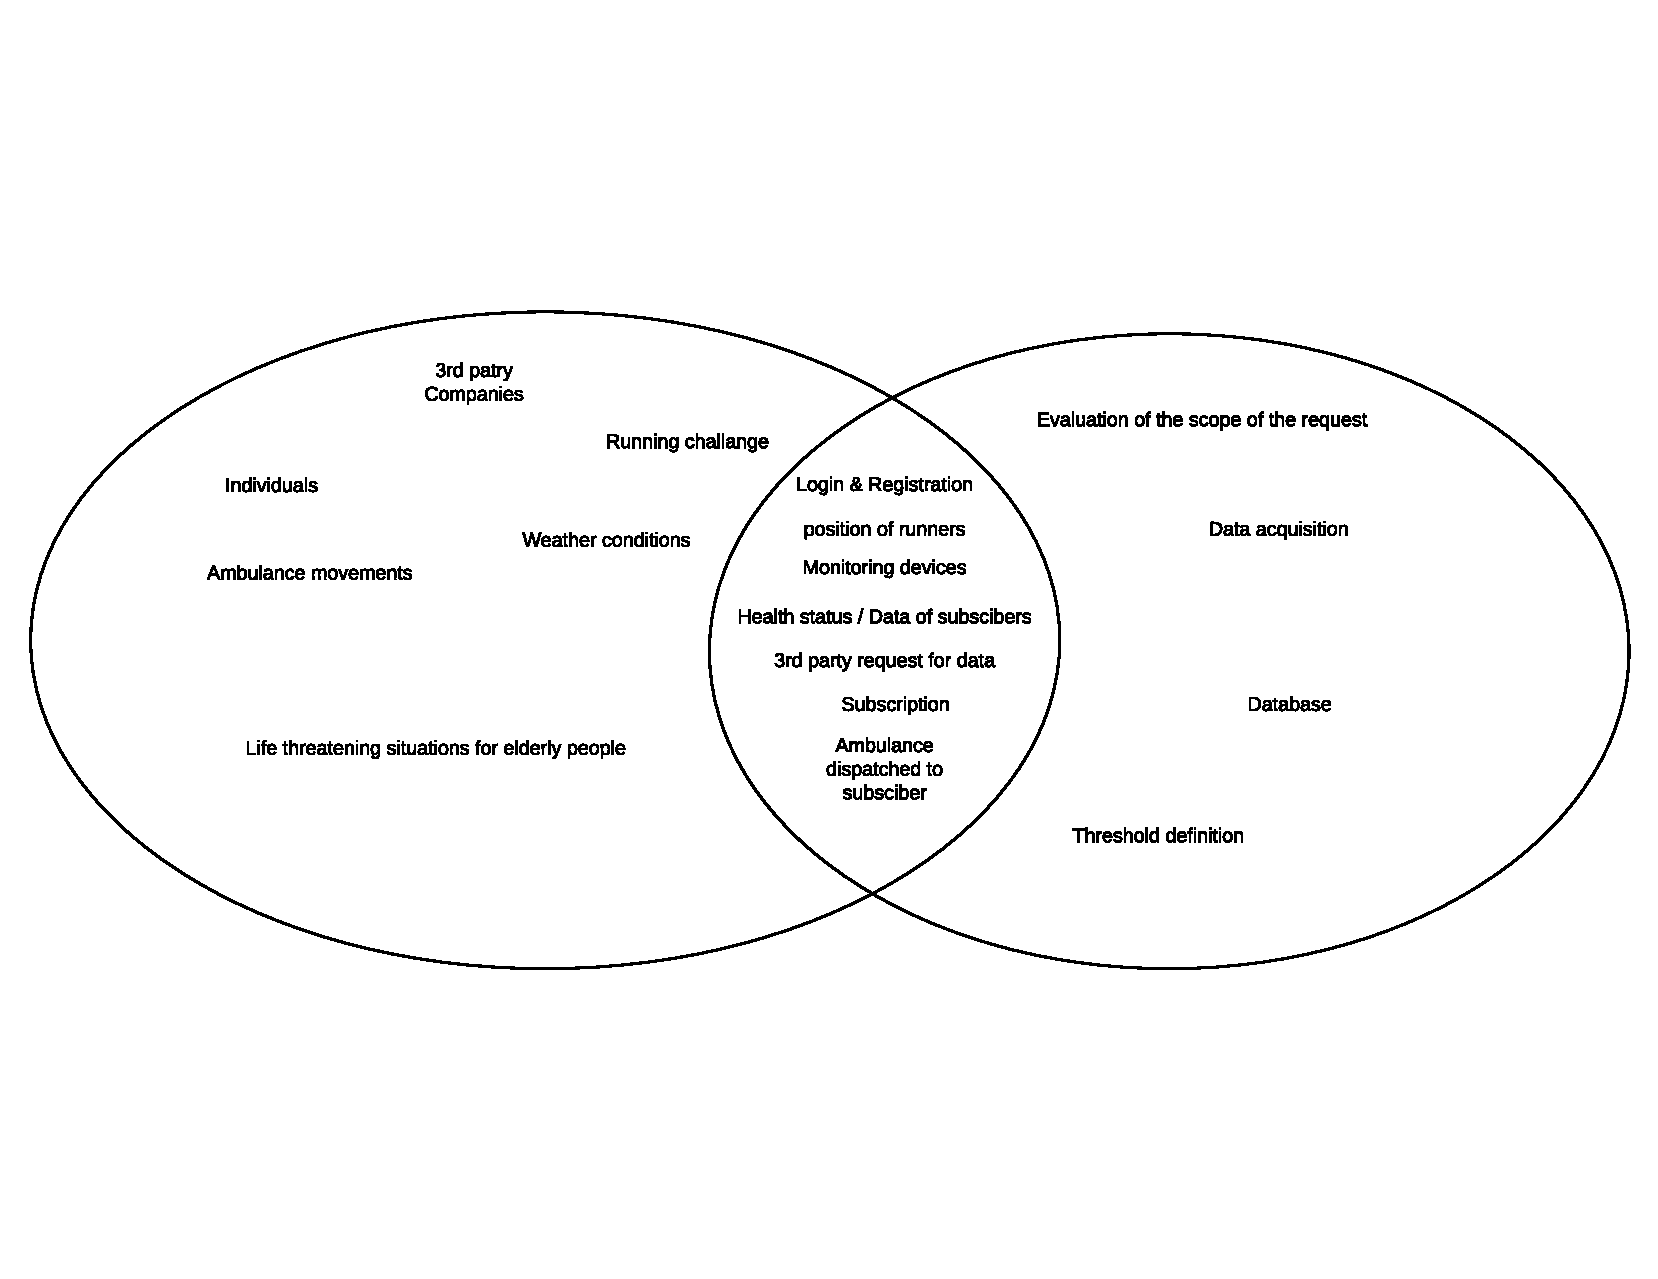
\includegraphics[height=8cm,keepaspectratio]{assets/twatm.pdf}
\end{center}

The system-to-be uses 3 components with different roles in order to work:
\begin{itemize}
    \item \textbf{Data4Help SmartWatch App}: Acquires the data from the smartwatch sensors (heart rate, sleep quality, position, phisical activities) and sends them via Bluetooth to the Data4Help Mobile App
    \item \textbf{Data4Help Mobile App}: Gathers data from the smartwatch, shows various statistics, and sends them to the Data4Help Core Database. Each user can choose which service subscribe to
    \item \textbf{Data4Help Website}: Gives third-party companies the ability to request data, either anonymized or user specific.
    \item \textbf{Track4Me Core}: is intended to connects all other components together providing the logic of the application. It is also responsible for the acceptance of all third-parties requests of data. It also evaluate health status of individuals deciding whether is at risk or not.
\end{itemize}

The list below shows the main goals the system should be able to accomplish:

\begin{itemize}
    \item \textbf{G1}: 
\end{itemize}

%A health data aggregator app that gives the user the ability to monitor all 

%is intended to offer all the functionalities of the service to the individuals, including heart rate monitoring, sleep monitoring

%% Add As a reference
% The world and the machine - paper
% http://mcs.open.ac.uk/mj665/icse17kn.pdf
